\section{Contributing}
Everyone is welcomed to contribute, but since this is a project made for students taking the \href{https://www.ntnu.edu/studies/courses/TDT4102}{TDT4102} NTNU course, their pull requests and issues will be prioritized. A detailed description on how to contribute will follow below.

\begin{enumerate}
    \item First, you'll need to fork the \href{https://github.com/LasseNatvig/SimComp}{\textit{Github}} repository by click on the "Fork"-button.
    \begin{figure}[H]
        \centering
        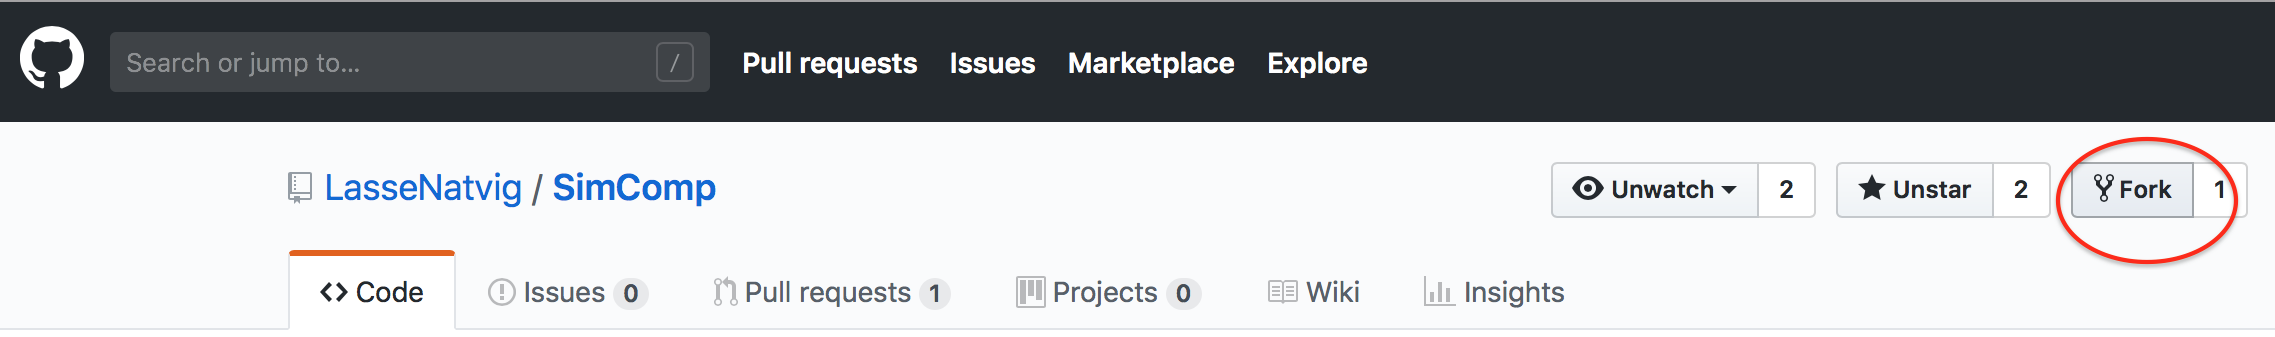
\includegraphics[scale=0.3]{img/Fork.png}
        \label{fig:fork}
    \end{figure}
    This will create version of the project on your \textit{Github}-account. 
    \item Next, follow section \ref{nedlasting} but replace the url in step 4 (3 on Linux/mac) with your own \texttt{https://github.com/<YOURUSERNAME>/SimCom.git} to download the project.
    \item Make changes to your version. Remember to push the changes to the remote (Github).
    \item Create a new pull request by click the "New pull request"-button in your fork. 
    \begin{figure}[H]
        \centering
        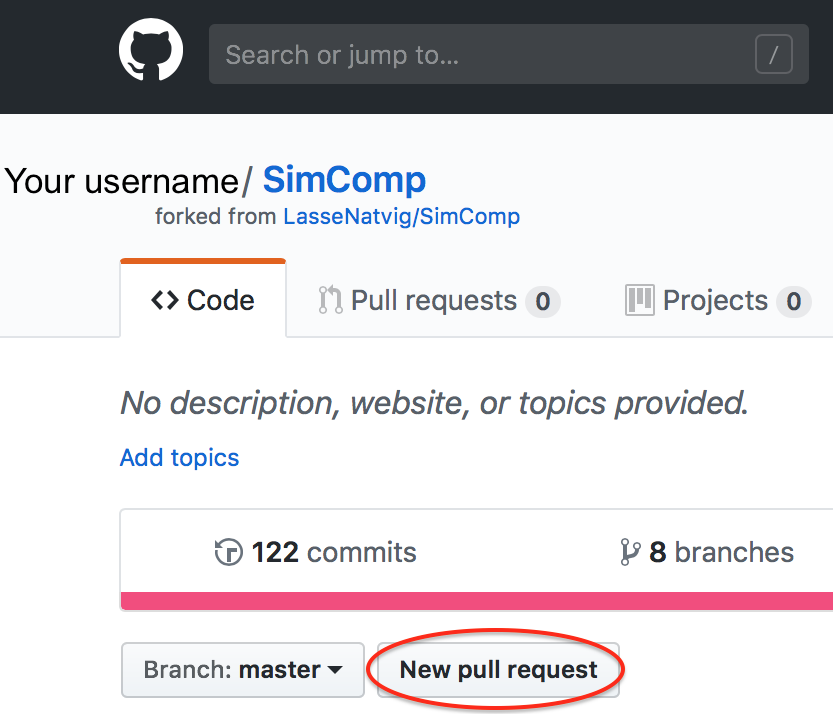
\includegraphics[scale=0.3]{img/Newpullrequest.png}
        \label{fig:fork}
    \end{figure}
    \item 
\end{enumerate}

